\chapter{Future Plans}
\noindent \rule{6.6in}{0.01in}
\vspace{0.5cm}

The progress achieved during the first semester has successfully established a highly efficient, bandwidth-conscious, decentralized workload forecasting backbone. Building upon this validated APSM framework, the roadmap for the second semester will focus on two major parallel tracks: extreme network scaling and the integration of autonomous Agentic Artificial Intelligence.

\section{Scaling to Massive Edge Topologies}
The initial Phase 1 evaluations provided robust proof-of-concept validation on a 10-node network. However, real-world edge computing architectures, particularly those utilized by telecommunications providers and smart city grids, are orders of magnitude larger. 

A primary objective for the next phase is to scale the custom discrete-event simulator to evaluate \textbf{50-node and 100-node peer-to-peer networks}. Scaling to these massive topologies will allow for a comprehensive stress-test of the APSM filter's mathematical resilience. Specifically, this phase will seek to definitively prove that as the network diameter expands, the ~50\% bandwidth suppression rate remains stable without inducing cascading accuracy failures across distant nodes. Running on 50 and 100-node topologies will also facilitate the calculation of precise, system-wide energy conservation metrics, providing a concrete environmental and economic justification for the protocol at scale.

\section{Transitioning from Passive Forecasting to Active Agentic AI}
The ultimate vision of this MTP is not merely to forecast workloads, but to actively orchestrate them. Standard DFaaS environments currently rely on passive, rule-based load balancers. Drawing inspiration from recent advancements in Multi-Agent Reinforcement Learning (MARL) for cloud-native clusters \cite{yao2025multi}, Semester 2 will introduce an \textbf{Agentic AI Orchestration Framework} deployed directly onto the edge nodes.

Instead of passively viewing the workload forecasts, autonomous AI agents will be initialized at each node. These agents will actively ingest the time-series predictions generated by the LSTM models and execute complex, goal-driven behaviors without human intervention. The future research vectors for the Agentic AI integration include:

\begin{itemize}
    \item \textbf{Autonomous Resource Negotiation:} When an agent's local LSTM model predicts an imminent spike in incoming workloads that exceeds the node's CPU capacity, the agent will autonomously initiate a negotiation protocol with neighboring agents. By preemptively securing offloading contracts, the network can seamlessly absorb massive traffic spikes without dropping serverless functions.
    \item \textbf{Dynamic Semantic Tuning via Reinforcement Learning:} The current APSM filter relies on a static sensitivity multiplier ($K=2.0$). In the next phase, Reinforcement Learning (RL) agents will be introduced to dynamically tune the $K$ parameter in real-time. If an edge node detects critically low battery levels, the local AI agent can autonomously increase $K$, further suppressing transmissions and sacrificing a marginal degree of forecasting accuracy in exchange for prolonged device survival.
    \item \textbf{Resilience and Self-Healing:} The agents will be tasked with identifying malicious nodes or sudden network partitions. By correlating the semantic surprise metrics ($\epsilon$) with historical peer behavior, agents can autonomously sever connections with corrupted nodes and establish new overlay links, ensuring self-healing topological resilience.
\end{itemize}

By merging the hyper-efficient APSM Gossip Learning foundation with proactive Agentic AI orchestration, the final thesis aims to present a holistic, next-generation architecture for fully autonomous, decentralized edge computing.

\vspace{1cm}
\begin{figure}[!ht]
    \centering
    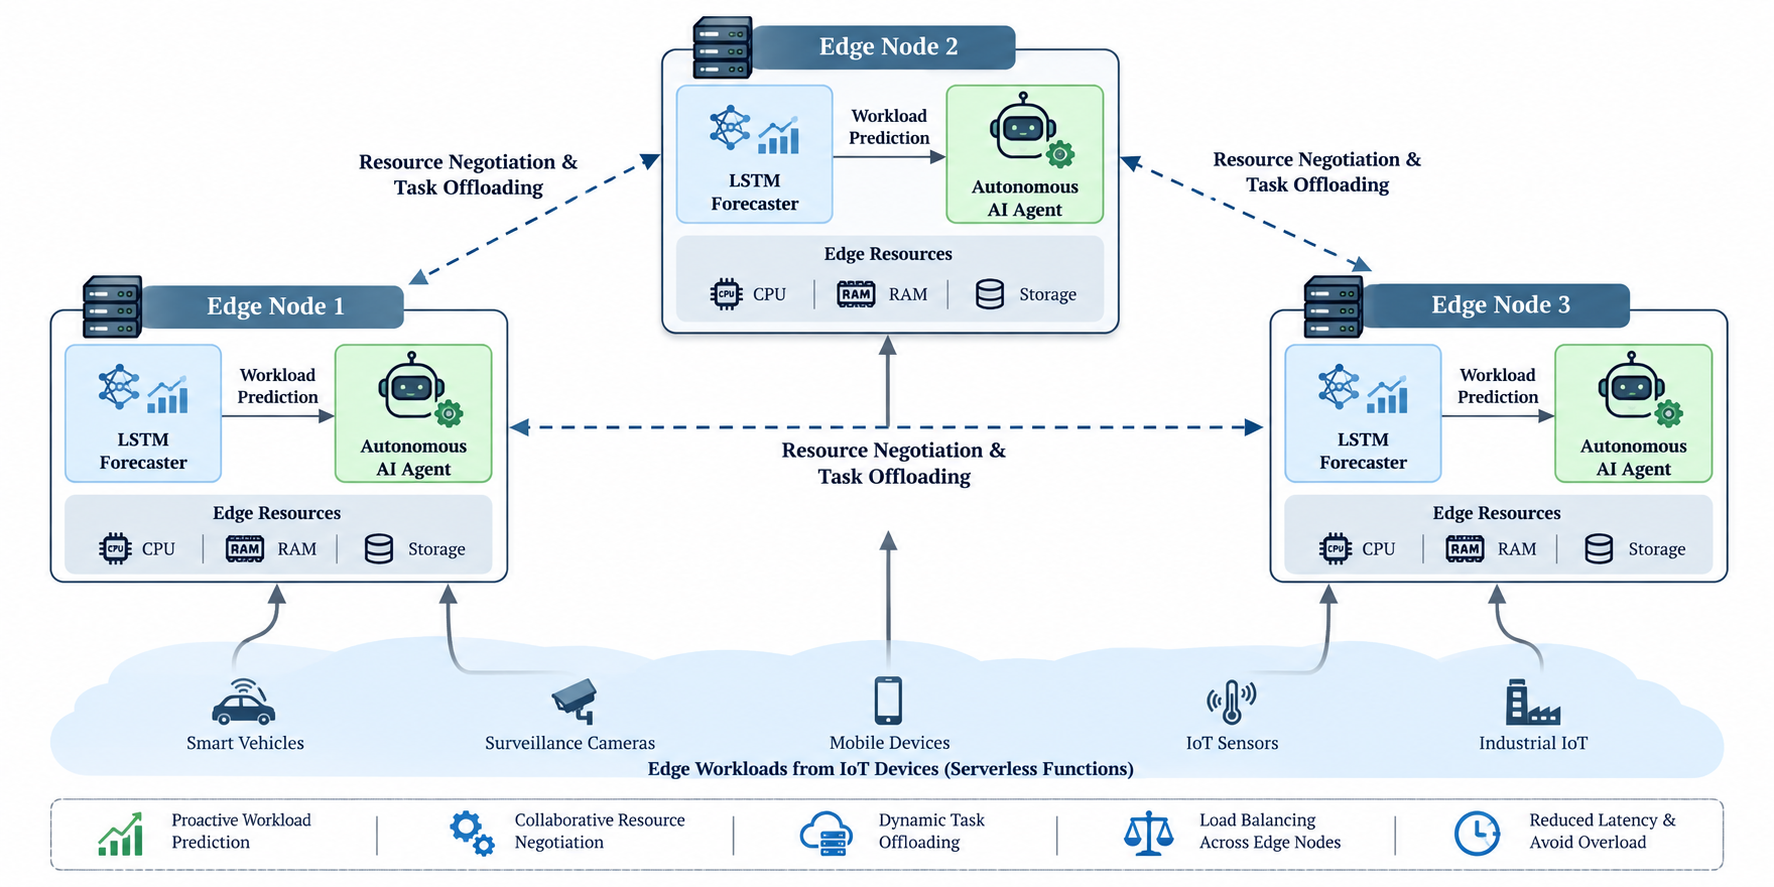
\includegraphics[width=0.6\textwidth]{chapters/figures/agentic_ai.png}
    \caption{Roadmap for Semester 2: Integration of Agentic AI for proactive edge orchestration.}
    \label{fig:future_plans}
\end{figure}
